\part{CODEC}

Para realizar aplicaciones con audio en la placa XSB Board \cite{XSBBoard} de que se dispone en el laboratorio de la asignatura, el primer paso a dar es realizar un driver en hardware para el codec\footnote{En este caso un codec se refiere a un conversor analógico-digital y otro digital-analógico, ambos estéreo, y no de un codificador-descodificador en el sentido de conversión entre formatos. A lo largo de la memoria en ocasiones se nombrará a los conversores como ADC y DAC respectivamente.} de audio que incluye dicha placa, concretamente el ASAHI KASEI AK4565 \cite{AK4565}.

	
	
\section{Desarrollo seguido}

	\subsection{Estudio de datasheets}
		El primer paso del desarrollo fue el estudio de los datasheets, tanto del codec como el de la placa. Del documento de la placa se obtuvo principalmente qué pines de la FPGA se conectaban con el codec y otros periféricos y en qué manera, lo cual puede verse resumido en la siguiente tabla:


\begin{figure}[H]

\centering
	\begin{tabular}{|c|c|c|c|c|}
		\hline
		\textbf{FPGA pin} & \textbf{Net name} & \textbf{Codec pin} & \textbf{Prog. Osc. pin}\\
		\hline
		141 (D2) & PB-D2 & CDTO &\\
		\hline
		145 (D1) & PB-D1 & CDTI &\\
		\hline
		153 (DIN/D0) & PB-D0 & CCLK &\\
		\hline
		165 & AU-CSN\# & CSN\# &\\
		\hline
		166 &  AU-BCLK & BCLK &\\
		\hline
		167 &  AU-MCLK & MCLK &\\
		\hline
		168 &  AU-LRCK & LRCK &\\
		\hline
		169 &  AU-SDTI & SDTI &\\
		\hline
		173 &  AU-SDTO0 & SDTO0 &\\
		\hline
		77 (I/GCK1) & FPGA-CLK1 & & CLKD\\
		\hline
	\end{tabular}

  \caption{Relación de conexiones entre FPGA, codec y oscilador programable.}
\end{figure}


	Del datasheet del codec vimos cuál era su funcionamiento de  manera general y más concretamente las palabras de configuración a cambiar y especificaciones técnicas como:

	\begin{itemize}
		\item Máxima resolución: 20 bits
		\item Máxima frecuencia de muestreo: 50 KHz
		
	\end{itemize}

	En las siguientes secciones se irá explicando con más detenimiento y se verán los detalles relevantes del codec, por lo que no repetiremos la información aquí.


	\subsection{Reloj principal}
		La placa dispone de un reloj de 100 MHz, con un divisor programable en enteros. Pensamos que el diseño que fuésemos a realizar, no sería capaz de funcionar a dicha velocidad por lo que intentamos el siguiente paso inferior, es decir, 50 MHz mediante un divisor de 2. Si este no fuese suficientemente lento, seguiríamos reduciendo la velocidad, sin embargo, no fue necesario.\\
		


	\subsection{Relojes para el codec}

		El codec necesita cuatro relojes diferentes: MCLK, CCLK, LRCK y BCLK. Para generarlos, creamos un módulo que partiendo del reloj global (clk) de 50 MHz, genere los cuatro mediante divisiones. (IS2CLOCKS.vhd).\\
		

		LRCK debe ser de frecuencia fs puesto que indica el canal con el que se está trabajando, MCLK de 256 o 384 (el codec detecta automáticame cuál tiene por lo que nosotros usamos 256 fs por sencillez) y BLCK, el reloj de bit, debe ser $>$40 fs para soportar la máxima resolución de 20 bits (nosotros usamos 64 fs de nuevo por sencillez).\\

		Dado el límite de muestreo del codec de 50 KHz, intentaremos que fs se aproxime todo lo que podamos a él sin pasarse. Todo ello puede realizarse con un contador con índice q y tomando como salidas de relojes lo siguiente:

		\begin{verbatim}
		MCLK <= q_i(1); -- CLK (50 MHz) / 4 = 12.5 Mhz = 256xfs
		BCLK <= q_i(3); -- CLK (50 MHz) / 16 = 3.125 Mhz = 64xfs
		LRCK <= q_i(9); -- CLK (50 MHz) / 1024 = 48.828 KHz = fs
		\end{verbatim} 

CCLK, el reloj de configuración, soporta hasta 5 MHz por lo que reutilizamos BCLK de 3.125 MHz.\\

		Siempre que es necesario utilizar uno de los relojes del codec dentro de la FPGA, en realidad no se usa directamente, si no que se utilizan eventos del reloj principal y se buscan cambios en los otros relojes para que todo el diseño sea síncrono y dependa de un único reloj.






	\subsection{Configuración o control del codec}

		Módulo CONTROL.vhd \textcolor{rosa}{(ESCRIBIR)}.

	
 
	\subsection{Loopback analógico}

		Configurando el codec para que tomase como entrada la conexión LINE IN y activando el loopback analógico incluido en el codec, comprobamos que el modulo que envía la configuración al codec funcionaba correctamente, puesto que ninguna de las dos opciones estaba configurada por defecto y tras arrancar la FPGA y mandar esta configuración, el audio que entraba por LINE IN llegaba a la salida.
		
	
	\subsection{Interfaz I$^2$S}

		El codec de audio permite utilizar varios interfaces de audio. De ellos elegimos I$^2$S por ser un estándar. Entonces, realizamos un módulo que se comúnicase con el codec utilizando este estándar para enviar y recibir información de audio (I2S.vhd). A partir de ahora, en vez de enviar la configuración de activación del loopback, enviamos la selección de I$^2$S como interfaz de audio.

	\subsection{Loopback digital}
		
		Para probar el módulo I2S que se encarga de la interfaz de audio, realizamos un modulo extremadamente sencillo consistente en unir las salidas del conversor digital-analógico con las entradas del conversor analógico digital de dicho módulo. El resultado es el mismo que el obtenido con el loopback analógico, pero ahora el audio está siendo convertido a digital en el codec, llevado a la FPGA, devuelto al codec y convertido de nuevo a analógico.

		

	
\section{Problemas encontrados}


	\subsection{Generación de relojes}
		Al principio pensamos que disponíamos de un reloj de 20 MHz, el margen de frecuencias generables era muy limitada  y además pensamos muestrear a 44100 Hz (frecuencia de muestreo de un CD), para ello implementamos divisores de doble módulo \cite{Fraccional divider in VHDL} que conseguían una frecuencia muy parecida en media pero con un \emph{jitter} impredecible. Abandonamos esta implementación al saber que el reloj del que disponíamos era de 100 MHz, y que podíamos aproximarnos con divisores enteros.

	

	\subsection{Canales cruzados}

		Quisimos comprobar que cada canal de audio (izquierdo y derecho) estaba siendo tratado como tal y no se estaban intercambiando. Para ello hicimos uso de archivos de audio lanzados desde el ordenador, de los cuales eramos capaces de distinguir con facilidad el canal izquierdo del derecho. Las pruebas que realizamos son las siguientes:

		\paragraph{Conexion sin cruzar canales}
			En esta prueba conectamos el canal izquierdo del ADC con el canal izquierdo del DAC, haciendo lo mismo con el canal derecho. Los canales se reproducían correctamente, cada uno en su respectivo lado.


		\paragraph{Conexion cruzando canales}
			En esta prueba conectamos el canal izquierdo del ADC con el canal derecho del DAC y el canal derecho del ADC con el canal izquiero del DAC. Los canales se reproducían cruzados, es decir, por el canal izquierdo se escuchaba el derecho y viceversa, como era de esperar.\\

En este momento llegamos a la conclusión, que más tarde se verá errónea, de que los canales eran tratados de forma correcta. Una imagen que ilustra lo que sucede en la placa es la siguiente:
\begin{figure}[h]
\begin{center}
	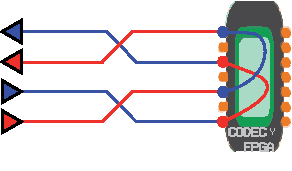
\includegraphics[width=0.5\textwidth]{./swapping_channels-eps-converted-to}
\caption{Cruce tanto a la entrada como a la salida de los conectores jack}
\end{center}
\end{figure}

		\paragraph{Utilización de un sólo canal de entrada y procesado diferente en cada canal de salida}
	
			Más tarde, ya trabajando con una aplicación que hacía uso del codec de audio realizabamos el siguiente montaje: tomabamos el canal izquierdo del ADC y lo envíabamos sin procesar al canal izquierdo del DAC y procesado al canal derecho del DAC.\\

La sorpresa era que el canal del que se tomaba el audio era el derecho en lugar del izquierdo y que se oía procesado el izquierdo en vez de el derecho.\\

Entonces pensamos que se cruzaban los canales de audio tanto en la etapa analógica-digital como en la digital-analógica. Esto está en concordancia con las anteriores pruebas hechas ya que en el caso de la conexión sin cruzar, puesto que se cruza en ambas etapas, finalmente cada canal está en el lado correspondiente.\\

Haciendo un cruce de canales al nivel de aplicación, tienen que escucharse cruzados porque se producirá un numero de cruces impar.\\

Por tanto, las pruebas que habíamos hecho antes y con las cuales habíamos pensado que el tratamiento de los canales era el correcto, no eran suficientes.\\

A partir de este momento dedicamos muchísimo tiempo a revisar nuestro código, repetir las simulaciones por si habíamos descuidado algún aspecto, volver a leer los datasheets, etc.\\

En el datasheet del codec vimos que la asignación de canales en relación a la señal LRCK (LEFT-RIGHT CLOCK) cuando se usa la interfaz I$^2$S es la contraria al resto de interfaces. En I$^2$S es LEFT=0, RIGHT=1 y en las demás, LEFT=1, RIGHT=0. Por tanto pensamos que la parte de control que envía la configuración al codec, podía estar mal, no estar seleccionándose I$^2$S y por ello estar los canales cruzados.\\

Repetimos las pruebas del módulo de control probando diferentes configuraciones y parecía que el no problema no se encontraba allí.\\

Comprobamos los esquemáticos de la placa para ver si el canal izquierdo estaba conectado a la punta de los jacks y  el derecho al contacto central. En los esquemáticos de nuevo era correcto, por lo que seguíamos sin saber cuál era la causa de los cruces de canales.\\

Finalmente, tomamos un multímetro y realizamos medidas sobre la placa para ver si la realidad se correspondía con los esquemáticos y no era así. En la placa, en realidad, el canal derecho estaba conectado a la punta del jack y el izquierdo al contacto central. Como esto ocurría tanto en el jack de entrada como en el de salida, se producía el doble cruce que antes describíamos.\\

Para solucionarlo, ante la evidente imposibilidad de modificar la placa, hicimos que dentro del módulo principal del driver del codec (I2S.vhd) se cruzasen los canales para tener todo como debería ser.
		
	

	
